% !TEX root = NSF_SuperCDMS_SNOLAB_OPS.tex
\section{Underground Test Facilities}
\label{sec:nexuscute}

A large part of this proposal is to perform critical measurements that require lower background environments than what has been available at our collaboration's surface test facilities. When operated at the surface, large cryogenic detectors can become swamped with cosmogenic background. Detailed detector performance properties, such as their discrimination power and behavior in the actual experimental environment, cannot be tested at surface facilities.

In this section we introduce two new underground sites that will be central to a large fraction of this work. The Cryogenic Underground TEst facility (\cute) is being built by the \SuperCDMS group at Queen's University and will be situated at \SNOLAB. The Northwestern EXperimental Underground Site (\nexus) is being built by the Northwestern University group and will be located in the MINOS near-detector hall at Fermilab. 

At the core of each facility is a cryogen-free dilution refrigerator equipped with special provisions to minimize the level of vibrations that may be introduced by the pulse tube cooler that provides the cooling down to 4~K. Both refrigerators provide a large cold volume that can house a SuperCDMS tower with a full complement of 6 detectors, and both are surrounded by a passive shield to lower radiogenic backgrounds. The two facilities are complementary. With a target background rate of $\sim$2~events\perkkd, \cute will offer lower overall backgrounds and radon mitigation, allowing for production \scs towers to be installed and tested. It is a low-background facility fully capable of cutting edge science. With a target background rate of $\sim$100 events\perkkd, \nexus is better described as a prototyping and R\&D facility, with less stringent background controls but more flexibility in its configuration and accessibility. Both still qualify as low-background environments when compared to surface facilities, which have a background rate of $\sim 10^4$\perkkd. This is why a number of calibration and detector characterization studies can be performed at \nexus and \cute that would be difficult or impossible to perform at a surface installation.\MP{There is no discussion of nuclear recoil backgrounds}.

\MP{Shouldn't we say that wiring / readout / grounding schemes / DAQ for these underground facilities is identical to that of SuperCDMS. A huge part of our argument is that work at these 2 facilities minimizes commissioning time of SuperCDMS SNOLAB}

\subsection{CUTE}
\label{sec:cute}

The \cute facility will be located in the Ladder Lab at \SNOLAB, next to the \SuperCDMS experiment. The cosmogenic background is therefore negligible, making the radiogenic backgrounds at \cute dominant. The dilution refrigerator will be placed inside a dry-well in the center of a water tank with a diameter of about 3.7 m and a height of about 3.2 m. The water acts as shielding material against external gamma and neutron radiation \MP{it's ultrapure water sourced from SNO right?}. The water layer thickness is about 1 m on the bottom and 1.5 m on the sides. The dry-well and the refrigerator itself generate an opening in the shielding on the top of the setup. Early Monte Carlo simulations for such a setup indicate an external gamma rate of order of 100 events\perkkd, strongly dominated by gammas entering directly from the top. In order to reduce the external gamma ray flux, and to protect the detectors from radiation that may originate from the dilution unit of the refrigerator, a 15 cm thick disk of lead is mounted inside the refrigerator, between the cooling unit and the detectors. The residual background for this setup was estimated to be a few tens of events\perkkd. The addition of an additional layer of lead inside the dry-well (15 cm at the bottom and 10 cm on the side walls, totaling $\sim$4 tons) is expected to reduce the external background by another order of magnitude. This background level of $\sim$2~events\perkkd\ allows for the measurement of the intrinsic \isotope[32]{Si} background in \scs detectors and opens the possibility of dark matter science prior to the start of \scs.

The \cute refrigerator has been ordered and is expected to be delivered to Queen's University for confirmation of performance in May 2017. The installation of the water tank and deck structure for access to the facility will begin in early 2017 so that the infrastructure is ready in summer 2017 when the refrigerator is expected to be delivered to \SNOLAB. The commissioning phase of \cute at \SNOLAB is expected to begin in late summer or early fall 2017.


\subsection{NEXUS}
\label{sec:nexus}

\begin{figure}
\centering
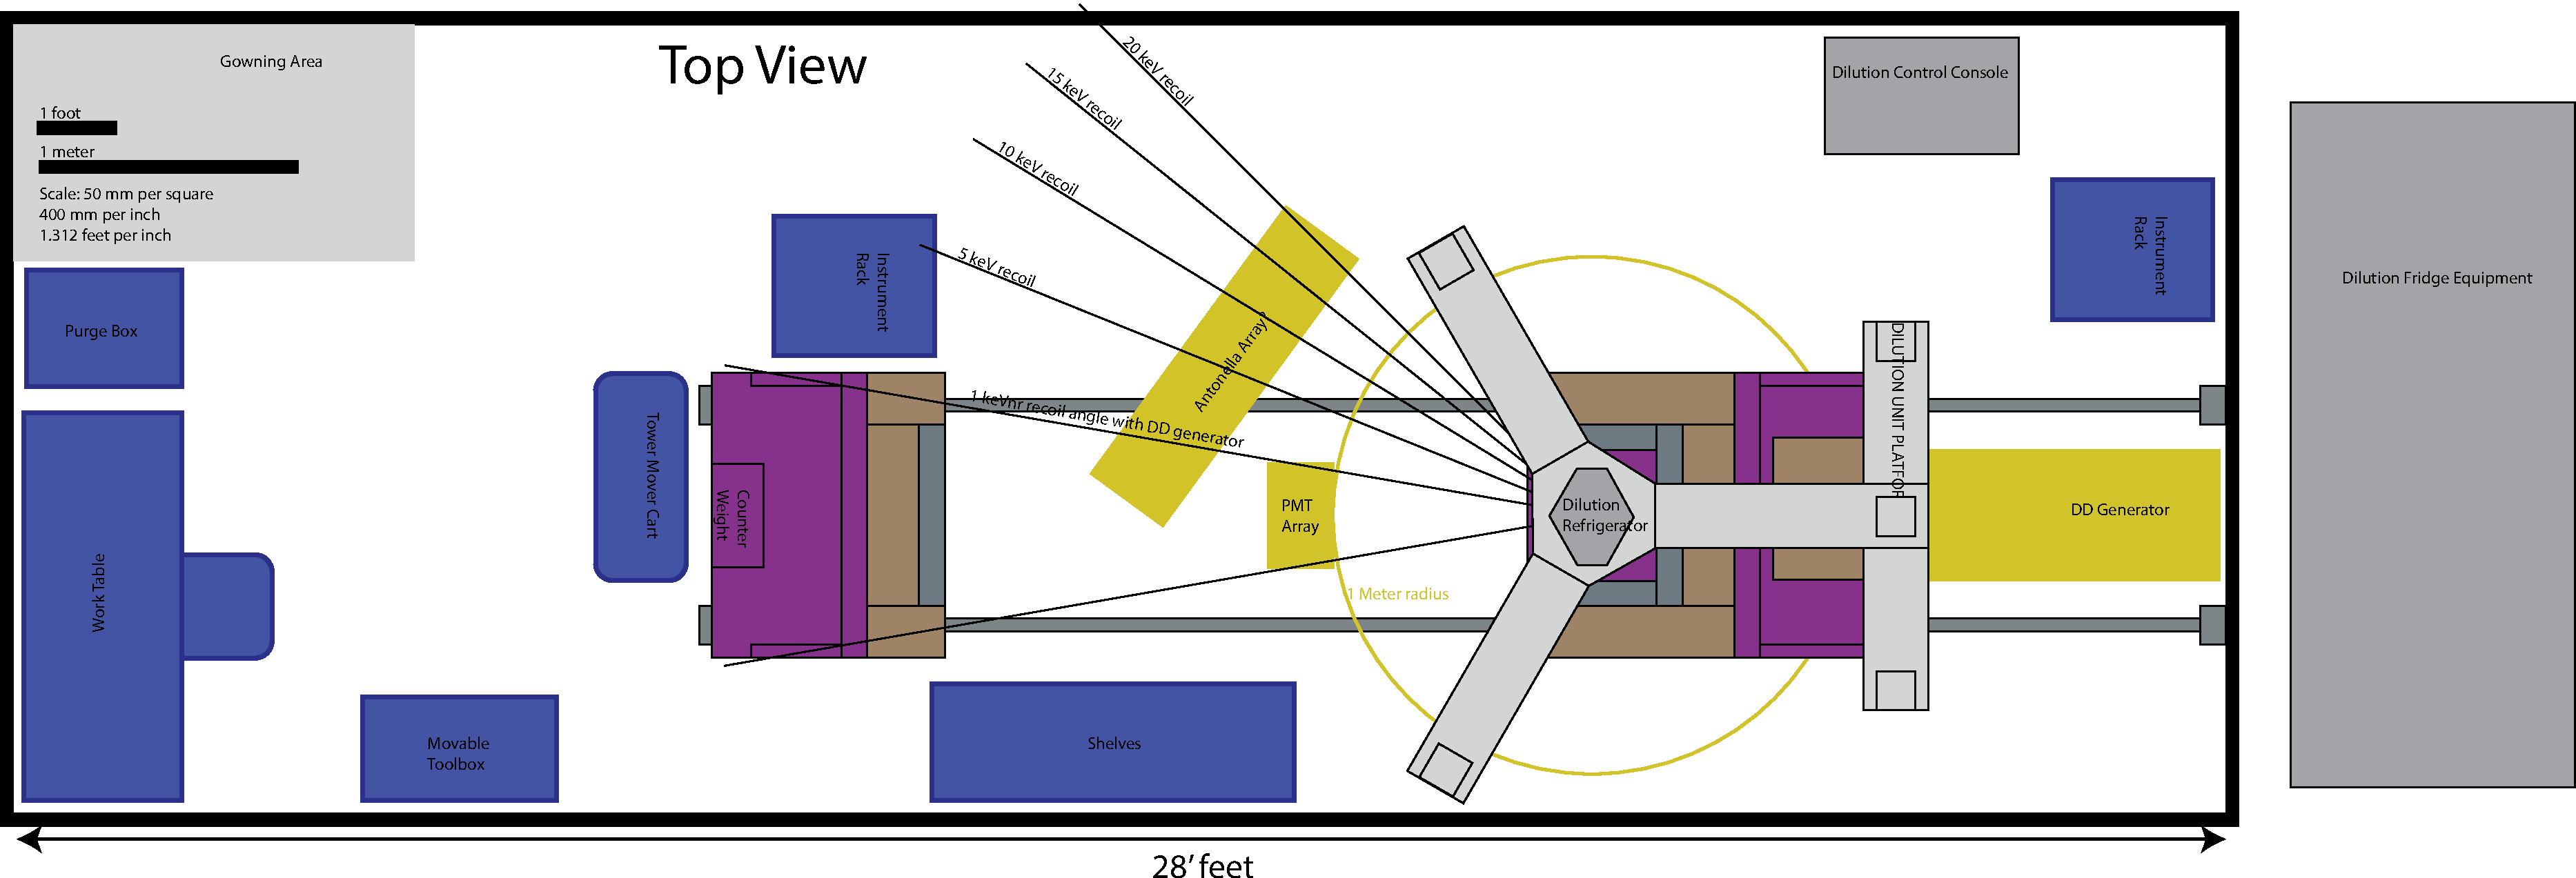
\includegraphics[width=\textwidth]{Figures/NEXUS-Layout-YieldMeas}
\caption{\nexus layout schematic. The outer box delineates the clean room to be placed 100 m underground in the \numi access tunnel. The blue boxes are support equipment, while the grey, brown, and purple structures are the passive shield, which is on rollers and half of it is moved out to the left to allow the neutron backing detectors to be placed. The D--D generator (described in Section~\ref{sec:ddcal}) is shown as a yellow box on the right, with neutrons passing through a collimating hole in the shield toward the detectors. Neutrons hit the HV detectors in the dilution refrigerator and scatter into angles as labeled depending on the recoil energy. An existing array from Fermilab will cover the wider angles between up to 20~keV, while a purpose-made fine-grain neutron detector PMT array will cover the recoil energies below 1~keV.\vspace{-2ex}}
\label{fig:nexus}
\end{figure}

\nexus is a testing facility planned for the MINOS near-detector hall at Fermilab ( 100~m underground). It will operate a dilution refrigerator surrounded by a 10~cm lead and 20~cm poly shield in a clean room environment. The rock overburden removes all muon-induced hadronic showers and lowers the muon flux to 0.5 muons/m$^2$/s. The lead shield (which includes a disk-shaped shield inside the refrigerator similar to \cute) will reduce the background to less than 100~events\perkkd. This facility is being built through a collaboration between Northwestern University and Fermilab.  A schematic of the calibration setup described in Section~\ref{sec:ddcal} is shown in Figure~\ref{fig:nexus}. The design of the clean room facility, the structural support for the dilution refrigerator, and the passive shield mechanical design are all underway. Installation of the dilution refrigerator is expected in fall of 2017, and the facility will be operational by the end of that year.


\subsection{Electronics and Shielding for \SuperCDMS Detectors}
%\comment{This probably belongs in the budget justification or somewhere else}

Much of the \scs hardware required to perform the measurements and science outlined in this proposal, such as pre-production towers and detectors, will be made available after the items are no longer needed for the \scs project. There are several exceptions, which are budgeted in this proposal and described here. To complete the measurements in this proposal at \nexus, the ability to read out two detectors is required. For \cute, a full contingent of 6 detector readout channels is needed for the science measurement. Thus we request: 

$\bullet$ Detector Control and Readout Cards (DCRCs). Two DCRC's are required to read out each HV detector, so we budget 4 for \nexus and 4 for \cute to test pre-production detectors. The HV tower will have its own DCRC's that will move to \scs with the tower.

$\bullet$ 300 K--4K wiring. The wiring to connect the DCRCs to the towers needs to be provided. Four are available for use at \cute, so we budget 8 more (we need 12 to read out the tower) and 4 for \nexus.

$\bullet$ Lead shield for \cute. The order of magnitude background reduction provided by this shield will provide sensitivity to the  \isotope[32]{Si} signal and the potential for early dark matter science. The shield for \nexus is already part of the facility.



